\section{GWT}
\label{subsec:gwt}

\begin{figure}[H]
    \centering
    
\includegraphics[scale=0.15]{images/gwt.png}
    \caption{Logotipo da framework GWT.}
    \label{fig:gwt}
\end{figure}

\hspace{5mm} A \href{http://www.gwtproject.org/}{\textbf{GWT}} consiste numa framework para construir e otimizar aplicações web complexas.

\hspace{5mm} Esta framework foi criada pela Google com o intuito de ser simples para os programadores desenvolverem a aplicação web e ser muito eficiente para os utilizadores. É uma framework client-side, apesar de ter um servidor a correr, este apenas serve para disponibilizar a view. Além disso esta framework não segue o modelo \textbf{MVC}, mas sim o modelo \textbf{MVP} (Model-View-Presenter).

\hspace{5mm} O \textbf{MVP} consiste em o utilizador interagir com a View, esta notifica o Presenter que por sua vez atualiza o Model, de seguida o Presenter obtém dados do Model e encaminha-os para a View para esta ser atualizada. A seguinte figura ilustra o funcionamento do modelo \textbf{MVP}.

\begin{figure}[H]
    \centering
    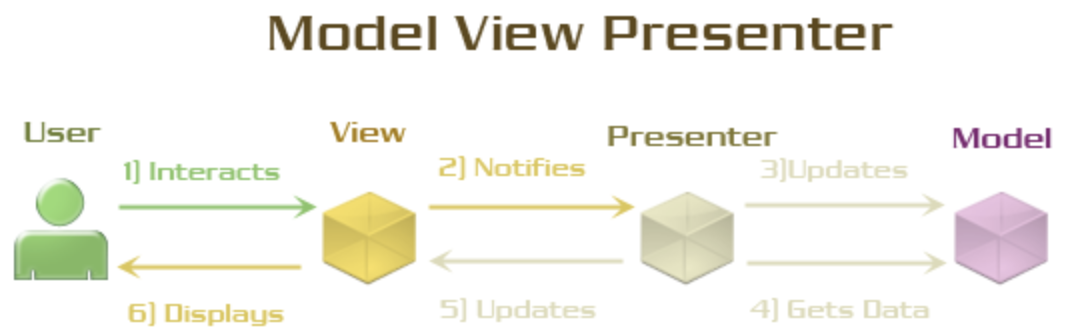
\includegraphics[scale=0.75]{images/MVP.png}
    \caption{Modelo \textbf{MVP}.}
    \label{fig:MVP}
\end{figure}

\hspace{5mm} Algumas das vantagens de utilizar o \textbf{GWT}:
\begin{itemize}
    \item Fornece API's Java e Widgets que permitem a escrita de aplicações AJAX em Java que depois são compiladas para JavaScript;
    \item Permite a colocação de "split-points" no código o que fará com que aplicações muito grandes possam ser divididas em vários segmentos JavaScript para um arranque mais rápido da página Web enquanto descarrega o resto dos fragmentos;
    \item Possui duas ferramentas de otimização para que o JavaScript gerado através do Java seja o mais eficiente possível, mas que também evite incompatibilidades entre diversos browsers;
    \item Os erros são encontrados em tempo de compilação;
    \item Pode ainda ser utilizado JavaScript entre o código Java através do JSNI (JavaScript Native Interface).
\end{itemize}

\hspace{5mm} De seguida será ilustrado um pequeno exemplo para mostrar a simplicidade da framework.

\begin{figure}[H]
    \centering
    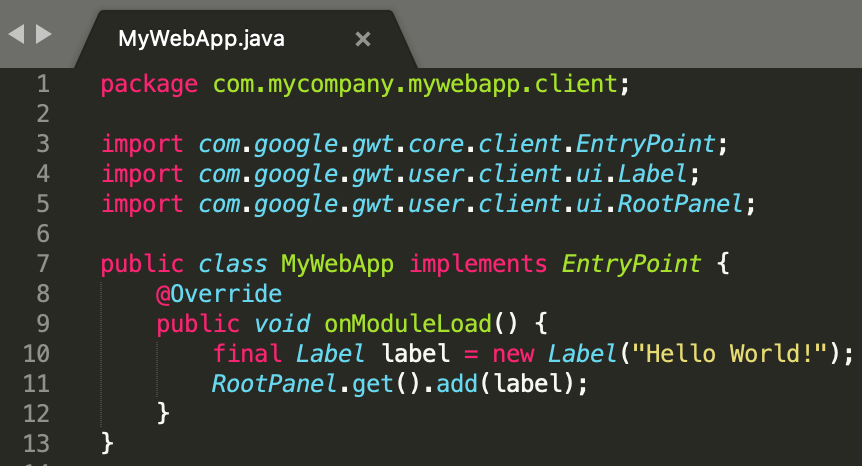
\includegraphics[scale=0.7]{images/gwt-1.png}
    \caption{Código Java para \emph{Quick Start}.}
    \label{fig:gwt-1}
\end{figure}

\begin{figure}[H]
    \centering
    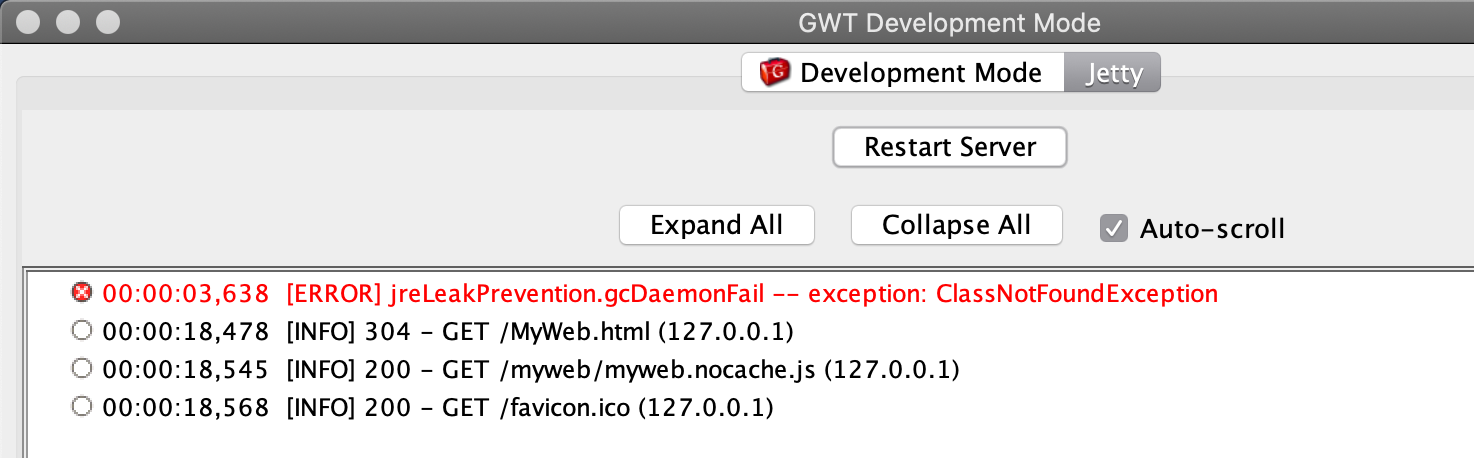
\includegraphics[scale=0.5]{images/gwt-2.png}
    \caption{Monitorização do servidor web, fornecida pela framework \textbf{GWT}, onde se pode ver os pedidos.}
    \label{fig:gwt-2}
\end{figure}

\begin{figure}[H]
    \centering
    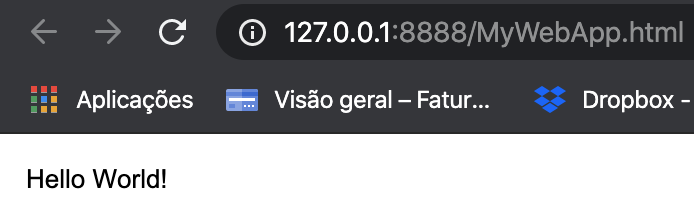
\includegraphics[scale=0.8]{images/gwt-3.png}
    \caption{A aplicação web criada pela framework.}
    \label{fig:gwt-3}
\end{figure}